\documentclass[10pt,norsk,a4paper]{article}
\usepackage[utf8]{inputenc}
\usepackage[T1]{fontenc}
\usepackage[norsk]{babel}
\usepackage[cm]{fullpage}
\usepackage{color}
\usepackage{parskip,textcomp,amssymb,graphicx}
\usepackage{pdfpages}
\usepackage[stable]{footmisc}
\usepackage{multicol}


\title{Ekstraordinær Generalforsamling \\
	Vår 2018\\[3cm]
	
\includegraphics[width=3cm,trim=0 4cm 0 0]{../res/logo.png}\\}
\date{28.\ februar 2018}
\author{Ifi-dagen}

% Blank header, samt footer med side x av y
\usepackage{fancyhdr}
\pagestyle{fancy}
\renewcommand{\headrulewidth}{0pt}
\fancyhead{}
\cfoot{Side~\thepage\ av~\pageref{lastpage}}



\begin{document}

\maketitle{}
\newpage
\tableofcontents{}
\newpage


\section{Valg av møteleder}

\section{Valg av referent}

\section{Valg av protokollunderskrivere}

\section{Valg av tellekorps}

\section{Godkjenning av innkalling}

\section{Godkjenning av dagsorden}

\section{Regnskap og revidert budsjett}
Økonomiansvarlig orienterer.
\subsection{Regnskap for 2017}

\subsection{Budsjett for 2018}

\section{Vedtektsendringer}
Følgende forslag til vedtektsendringer ligger fremme.

\subsection{Endringer i forbindelse med styret og generalforsamling}
Vedtektene angående oppbygging av styret er lite fleksible slik de er nå, samt at hvordan stemmeangivning foregår ikke er spesifisert. Styret kommer derfor med følgende forslag til vedtektsendringer:

\subsubsection{Forslag til endring av paragraf: §2--2b}
\begin{quote}
	\begin{enumerate}
		\item[§2--2b] Funksjonstiden for et styremedlem varer frem til neste ordinære generalforsamling.
		\item[§2--2b] Funksjonstiden for et styremedlem varer enten frem til neste ordinære generalforsamling, eller fram til utgangen av året som styret ble innvalgt for, hva enn som er lengst.
	\end{enumerate}
\end{quote}

\subsubsection{Forslag til endring av paragraf: §2--2c}
\begin{quote}
	\begin{enumerate}
		\item[§2--2c] Styret skal bestå av følgende verv: leder, nestleder, økonomiansvarlig, teknisk ansvarlig, to promoteringsansvarlige, underholdningsansvarlig, bedriftsansvarlig, faglig ansvarlig og funksjonæransvarlig.
		\item[§2--2c] Styret skal minimum bestå av leder, økonomiansvarlig og bedriftsansvarlig, og disse vervene kan kun velges på en generalforsamling.
	\end{enumerate}
\end{quote}

\subsubsection{Forslag til ny paragraf: §2--2d}
\begin{quote}
	\begin{enumerate}
		\item[§2--2d] Styret kan velge andre verv til valg før generalforsamlingen.
	\end{enumerate}
\end{quote}

\subsubsection{Forslag til endring av paragraf: §2--2d}
\begin{quote}
	\begin{enumerate}
		\item[§2--2d] Dersom enkelte verv ikke blir fylt på generalforsamling kan styret selv etterfylle nye styremedlemmer, med unntak av leder og økonomiansvarlig som må velges på ekstraordinær generalforsamling.
		\item[§2--2e] Dersom verv fra punkt d ikke er fylt etter generalforsamling, eller et styremedlem fratrer, kan styret selv etterfylle nye styremedlemmer som blir sittende til neste ordinære generalforsamling.
	\end{enumerate}
\end{quote}

\subsubsection{Forslag til ny paragraf: §2--2f}
\begin{quote}
	\begin{enumerate}
		\item[§2--2f] Valg av styremedlemmer på generalforsamling skjer ved Instant-runoff vote, også kjent som IRV, eller alternativ stemmegivning.
	\end{enumerate}
\end{quote}

\subsection{Endringer i forhold til FU}
Paragraf 4 ble spesifisert før man årlig gjennomførte ettermiddagen@ifi, som har gått i underskudd hvert år det har blitt arrangert. Derfor ønsker styret å sette opp egenkapitalen fra kr 100 000,– til kr 200 000,– for å sikre at foreningen har nok økonomiske midler til å gjennomføre ettermiddagen- og dagen@ifi, samt andre arrangementer som eventuelt blir holdt.

\subsubsection{Forslag til endring av paragraf: §4--1}
\begin{quote}
	\begin{enumerate}
        \item[§4--1] Ved innføring av nytt styre skal et eventuelt overskudd overføres til Fordelingsutvalget, foruten en egenkapital på kr 100 000,–. Fordelte midler skal gå til formål som kommer studentene ved Ifi til gode.
        \item[§4--1a] Ved innføring av nytt styre skal et eventuelt overskudd overføres til Fordelingsutvalget ved Institutt for informatikk, foruten en egenkapital for foreningen på kr 200 000,–.
	\end{enumerate}
\end{quote}

\subsubsection{Forslag til ny paragraf: §4--1b}
\begin{quote}
	\begin{enumerate}
		\item[§4--1b] Fordelte midler fra et eventuelt overskudd skal gå til formål som kommer studentene og deres studentforeninger ved Institutt for informatikk til gode.
	\end{enumerate}
\end{quote}\label{lastpage}

\newpage

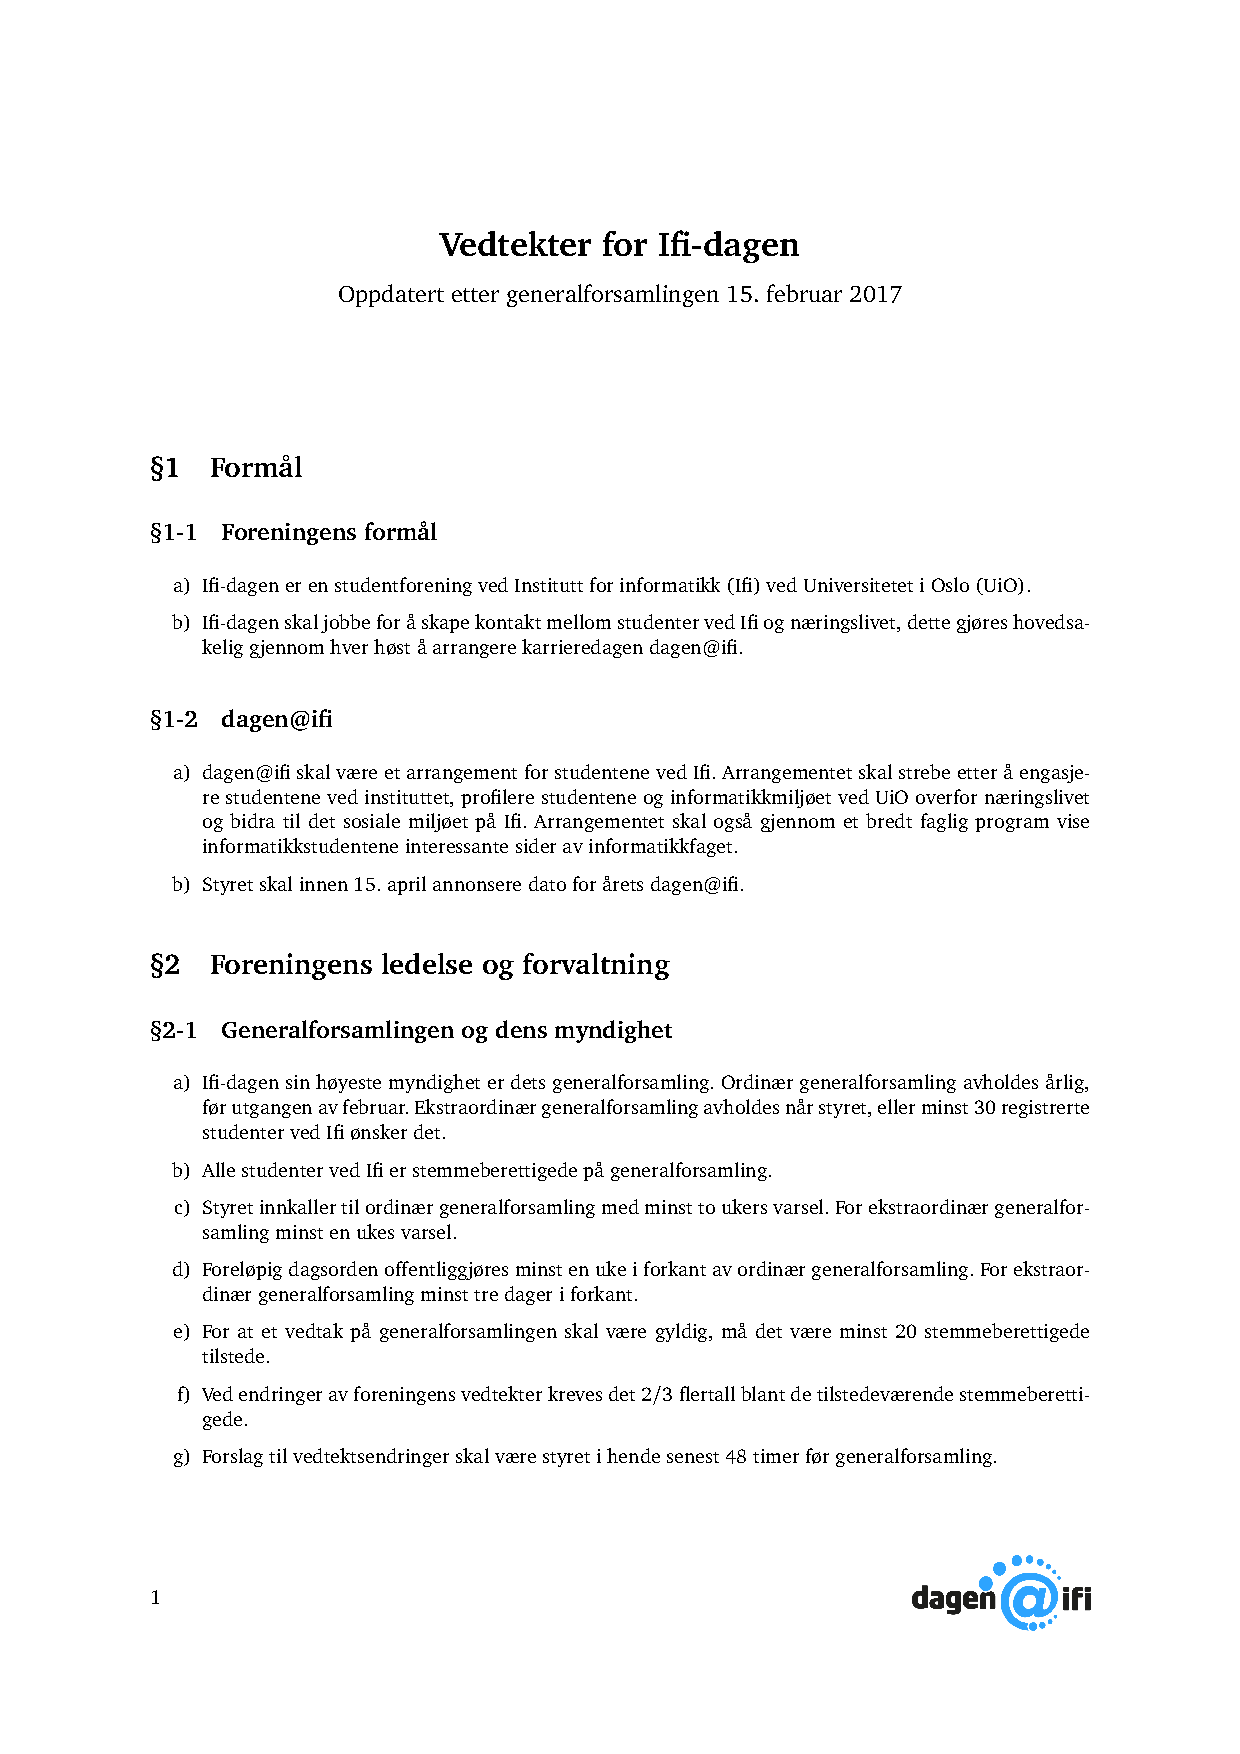
\includepdf[pages=-]{../vedtekter/vedtekter.pdf}
\end{document}
